%!TEX root = doc.tex
\section{\apiname{} Architecture} % (fold)
\label{sec:proposal}

At times, when developing MAS on a specific platform, a need arises for adopting different tools than those available in the original platform. More specifically, this paper is the result of a necessity to quickly and easily create JADE-based applications out of Repast-based simulations, eventually being able to perform the complementary operation. \apiname{}'s main goal is to enable in Repast the support for the development of FIPA-compliant MABS. In this section we try to give a thorough description of \apiname{}'s architecture while comparing our design decisions with those of JADE.
% [citation needed: is conversion a real need?]

\subsection{Repast and JADE}
% What was missing in Repast?
JADE and Repast are two popular agent-based application development tools with a very distinct set of features. Table \ref{tab:jadevsrep} summarizes the main differences between the two. It's worth pointing out that communication and ontologies are both covered by FIPA specifications. This, together with the differences in agent execution, make up the targets of out API.

Our goal is not to reproduce JADE's distribution architecture in Repast. One advantage of using Repast is that, since the communication is local (while JADE's agents are often spread in different containers), the execution of Repast-based simulations is typically much faster. This also makes it more suited to perform simulations and tests on MAS \cite{mengistu2008scalability} \cite{gormer2011jrep} \cite{garcia2011misia}.

By incorporating FIPA specifications in Repast, we bring it closer to JADE. By using \apiname{}, programmers that are already comfortable with creating MAS in JADE can feel comfortable enough to produce Repast-based simulations with the tools they're used to in JADE.

\begin{table}[h]
	\caption{Summary of JADE and Repast features.}
	\label{tab:jadevsrep}
	\begin{center}
		\begin{tabular}{l|cc}
		\hline

		\hline
		\textbf{} & \textbf{JADE} & \textbf{Repast} \\ %& \textbf{Cougaar} \\
		\hline
			Agent 		& FIPA  	&  Method calls  \\ %& Serialized Object \\
			Interaction	& protocols	&  Shared resources \\
		\hline
			Distribution & Yes & No \\ %& Yes \\
		\hline
			Simulation Tools & No & Yes \\ %& Yes \\
		\hline
			Scalability & Limited & High \\ %& High \\
		\hline
			Ontologies & Yes & No \\ %& Yes\\
		\hline
			Open Source & Yes & Yes \\ %& Yes\\
		\hline
			Agent  		& Behavior-based & Schedule-based  \\ %&  \\
			Execution	& Multi-threaded & Single-threaded \\ %&  \\
						& Event-driven   & Tick-driven 	   \\ %&  \\
						& Assync		 & Sync 		   \\ %&  \\
		\hline
		\end{tabular}
	\end{center}
\end{table} 

\subsection{FIPA Specifications}

As mentioned before, \apiname{} closely follows JADE's architecture regarding the use of protocols and services specified by FIPA. The architecture described in this paper includes three concepts proposed by FIPA: the Directory Facilitator (DF), the Message Transport Service (MTS) and the Interaction protocols.

The DF is a component that provides a yellow page service and is part FIPA Agent Management Specification \footnote{FIPA AM - http://www.fipa.org/specs/fipa00023/XC00023H.html}. It allows one agent to perform searches in order to request information about other agents. Only agents that are registered in the DF will be indexed and agents can register and deregister themselves at any time. These searches can be filtered in order to find the agents that are announcing themselves as providers or certain service. 

In \apiname{}, the services used as filters in search are the type of interaction behavior that an agent is expected to have adopted. Since the context of out tool is the development local (vs. distributed) simulations, a single DF exists in each simulation. Is worth noting that Repast has it's own agent manager, named ``Context''. \apiname{} offers support to this feature by integrating a reference to this object in the DF.

The MTS is a service, also specified by FIPA \footnote{FIPA MTS - http://www.fipa.org/specs/fipa00067/SC00067F.html}, for transportation of ACL messages between agents. One of its tasks is to be able to resolve agent addresses, in order to be able to deliver those messages. \apiname{}'s implementation of the MTS is simplified. Since \apiname{}'s target is the development of simulations in Repast, all our agents are local and agent address resolution is not required.

Finally, the main focus of the software we're proposing is the incorporation of FIPA Interaction Protocols in Repast. At the present time, we chose to include a few of the most common protocols in \apiname{}, following JADE's implementation.

The FIPA protocols from JADE we chose to include in \apiname{} at this point were the ``request-like'' Achieve Rational Effect (AchieveRE) protocol, the Propose protocol and the Contract Net protocol. The AchieveRE is a single protocol that encompasses multiple FIPA protocols, namely FIPA-Request, FIPA-query, FIPA-Request-When, FIPA-recruiting and FIPA-brokering protocols, as defined in JADE's documentation \footnote{http://jade.tilab.com/doc/api/jade/proto/AchieveREInitiator.html}.

\subsection{\apiname{} architecture}

\apiname{}'s implementation is essentially based on JADE. In the process of incorporating FIPA specifications, conceptual adaptations had to be made to reproduce Repast's the concept of time in JADE's protocols, which are essentially event-driven. In \apiname{}, communication happens asynchronously but not event-driven. As Figure \ref{fig:com-example} shows, agent execution in Repast in not concurrent. Repast uses a time-share type of execution, granting each agent the right to perform its tasks until they finish them, in sequence, but in no particular order. The figure represents a best case scenario where the order of execution of the agents by Repast was favorable to communication. It's not unexpected for Agents A and B to execute again once before Agent C does, making the protocol take a bit longer to finish.

\begin{figure}[h]
	\centering
	\includegraphics[width=3.0in]{figures/tickExample2.png}
	\caption{
		Communication example in JADE. Agents are executed concurrently or in parallel. Agent C handles messages as they arrive.
	}
	\label{fig:com-example-jade}
\end{figure}

\begin{figure}[h]
	\centering
	\includegraphics[width=3.5in]{figures/tickExample.png}
	\caption{
		Communication example in Repast using \apiname{} in a single tick. In their respective turns, A and B send a message to C, which stays in standby in C's Mailbox. Only in C's turn do these messages get handled.
	}
	\label{fig:com-example}
\end{figure}


Figure \ref{fig:arch} illustrates the details of \apiname{}'s architecture. Most concepts represented in this diagram are present in JADE, namely the Agent, ACL Message, Behavior, MTS and DF service.

An agent in \apiname{} contains a queue of Behaviors and a mail box. On each ``round'', these behaviors are schedules to be executed and some will take care of handling the messages arrived at the mail box.

The protocol package contains the implementation of different FIPA protocols. The ones ported from JADE were the ``Request-like'' Achieve RE, Propose and Contract Net. Other protocols can be created by extending these and creating new behaviors can be done by extending the main Behavior.

Analogous to JADE, the DF service in \apiname{} allows an agent to find other agents. It is possible to filter the agent search by service, i.e. specify what behaviors or protocols they should be executing. The MTS is a facility used for message delivery.


\begin{figure}[h]
	\centering
	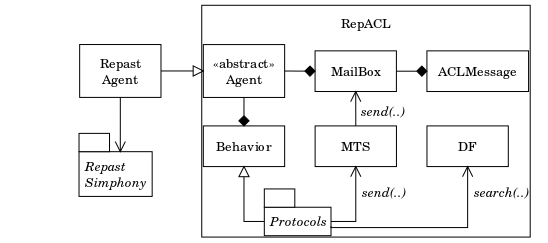
\includegraphics[width=3.5in]{figures/repacl_arch.png}
	\caption{Detailed architecture or \apiname{}}
	\label{fig:arch}
\end{figure}

% section proposal (end)